%!TEX root = ../thesis.tex
\section{構造解析}
設計したアームには,7つの板金部品を使用している.それぞれの部品は,軽量化と強度を考慮し設計している.特に,肩部の部品1と部品2(図\ref{fig:shoulder})は,最も負荷がかかる部位であるため,inventor上で構造解析を行い,強度を確認している.以下に,各部品の構造解析について述べる.
\begin{figure}[h]
  \centering
  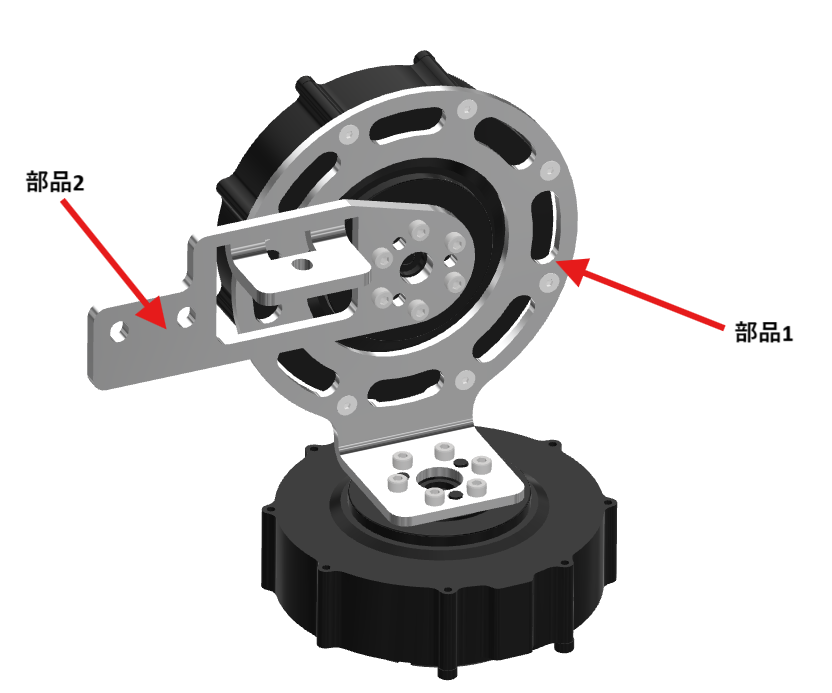
\includegraphics[width=10cm]{images/design/shoulder.png}
  \caption{Configuration of robot arm shoulder}
  \label{fig:shoulder}
\end{figure}
\clearpage
\subsection{部品1の構造解析}
部品1は,肩部のヨー軸モータの出力軸と,ピッチ軸モータを繋いでおり,アルミニウム合金(A5052)で加工されている.この部品に最大の負荷がかかるのは,ヨー軸が最大出力の22Nmで動作した時である.部品の重心位置に荷重が加わるとし,その時の部品の構造解析の結果を図\ref{fig:T3_40}に示す.また,この部品の厚み,質量,安全率を表\ref{tab:part1_spec}に示す.現状の設計では,安全率が0.39となっており,強度が不足している.
\begin{figure}[h]
  \centering
  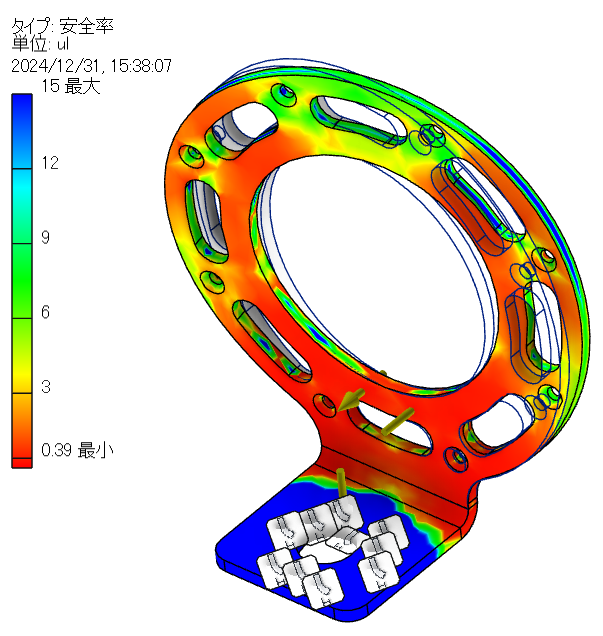
\includegraphics[width=6cm]{images/design/T3_40.png}
  \caption{Structural analysis results using Inventor of Part 1}
  \label{fig:T3_40}
\end{figure}
\begin{table}[h]
  \centering
  \begin{tabular}{lc}
    \hline
    \multicolumn{1}{c}{\textbf{厚み}} & 3㎜    \\ 
    質量                               & 43.6g \\ 
    安全率                              & 0.39  \\ \hline
  \end{tabular}
  \caption{Specifications of Part 1}
  \label{tab:part1_spec}
\end{table}
\clearpage
そこで,部品1の強度を向上させるため,形状を変えずに厚みを5㎜に変更した場合の構造解析を行った.その結果を\ref{fig:T5}に示す.また,同様に表\ref{tab:part1_spec_T5}にその時の部品の厚み,質量,安全率を示す.この設計では,安全率が1.01となり,強度が確保されている一方で,質量が71.1gとなり,重量が増加している.
\begin{figure}[h]
  \centering
  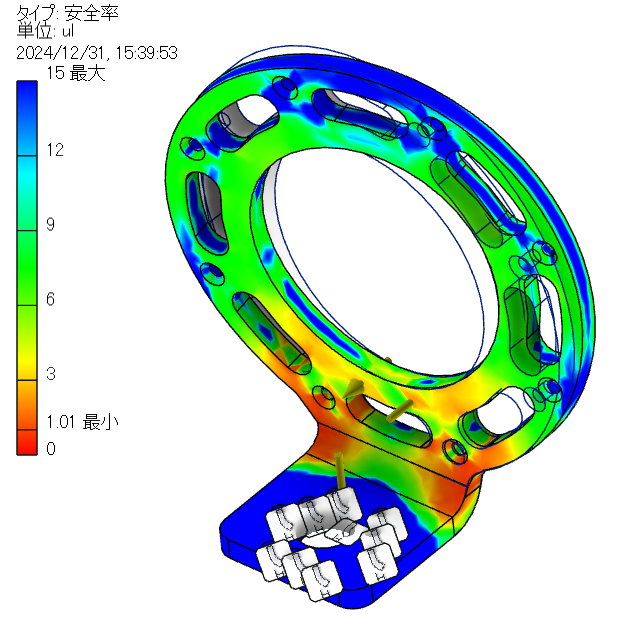
\includegraphics[width=6cm]{images/design/T5.png}
  \caption{Structural analysis results using Inventor of part 1 after changing the thickness}
  \label{fig:T5}
\end{figure}
\begin{table}[h]
  \centering
  \begin{tabular}{lc}
    \hline
    \multicolumn{1}{c}{\textbf{厚み}} & 5㎜    \\ 
    質量                               & 71.1g \\ 
    安全率                              & 1.01  \\ \hline
  \end{tabular}
  \caption{Specs of part 1 after changing the thickness}
  \label{tab:part1_spec_T5}
\end{table}
\clearpage
厚みを3㎜のままで強度を向上させるため,部品1の形状を変更した場合の構造解析を行った.その結果を図\ref{fig:T5}に示す.また,同様に表\ref{tab:part1_spec_T5}にその時の部品の厚み,質量,安全率を示す.この設計では,安全率が1.1となり,強度が確保されている.また,厚みを変更した時よりも質量が軽くなり,61.8gとなっている.
\begin{figure}[h]
  \centering
  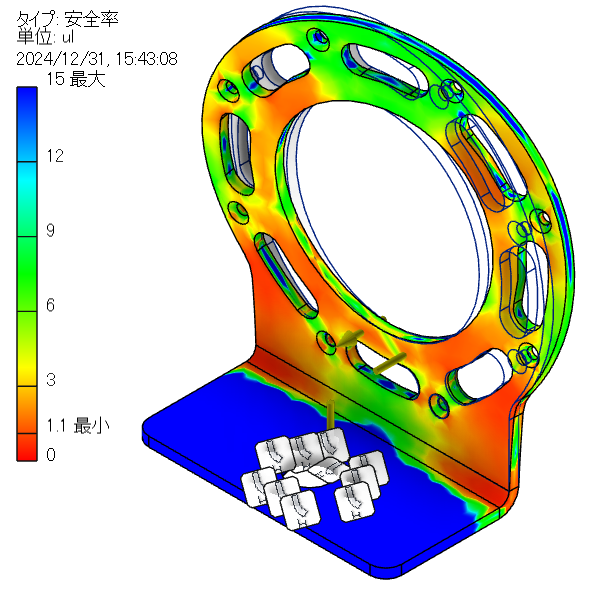
\includegraphics[width=6cm]{images/design/T3_80.png}
  \caption{Structural analysis results using Inventor of part 1 after changing shape}
  \label{fig:T5}
\end{figure}
\begin{table}[h]
  \centering
  \begin{tabular}{lc}
    \hline
    \multicolumn{1}{c}{\textbf{厚み}} & 3㎜    \\ 
    質量                               & 61.8g \\ 
    安全率                              & 1.1  \\ \hline
  \end{tabular}
  \caption{Specs of part 1 after changing shape}
  \label{tab:part1_spec_T5}
\end{table}
\clearpage
\subsection{部品2の構造解析}
\newpage